\documentclass{standalone}
\usepackage{tikz}
\usetikzlibrary{patterns, positioning}


\begin{document}
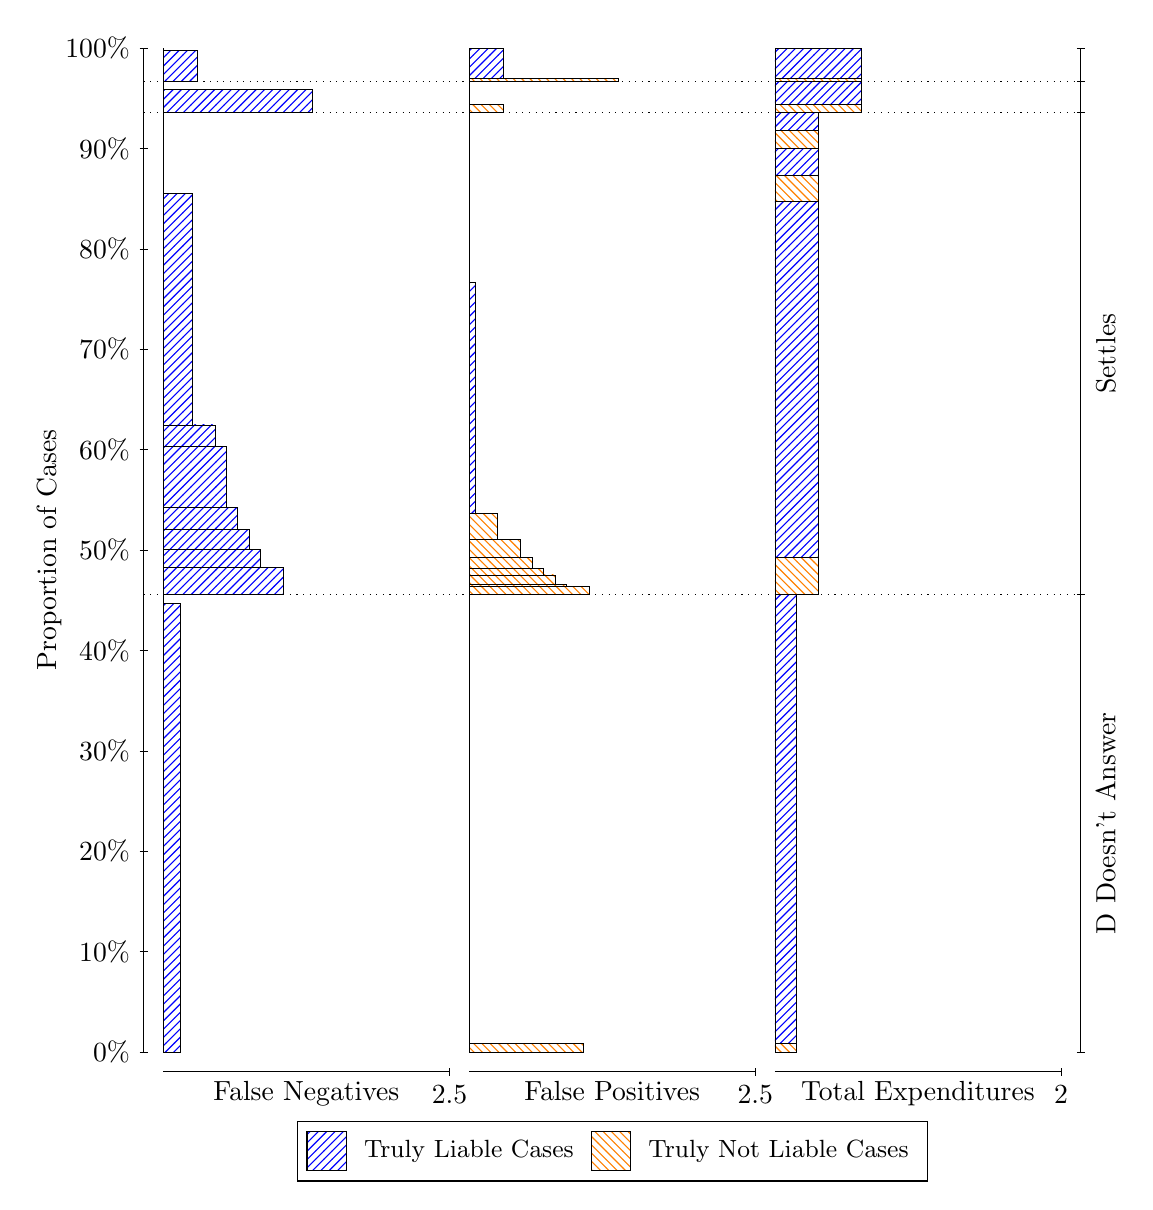
\begin{tikzpicture}
\draw[black, very thin] (1.5,1.75) -- (1.5,14.5);
\node[rotate=90, text=black, anchor=center] at (0.3, 8.125) {Proportion of Cases};
\draw[black, very thin] (1.45,1.75) -- (1.55,1.75);
\node[text=black, anchor=east] at (1.45, 1.75) {0\%};
\draw[black, very thin] (1.45,3.025) -- (1.55,3.025);
\node[text=black, anchor=east] at (1.45, 3.025) {10\%};
\draw[black, very thin] (1.45,4.3) -- (1.55,4.3);
\node[text=black, anchor=east] at (1.45, 4.3) {20\%};
\draw[black, very thin] (1.45,5.575) -- (1.55,5.575);
\node[text=black, anchor=east] at (1.45, 5.575) {30\%};
\draw[black, very thin] (1.45,6.85) -- (1.55,6.85);
\node[text=black, anchor=east] at (1.45, 6.85) {40\%};
\draw[black, very thin] (1.45,8.125) -- (1.55,8.125);
\node[text=black, anchor=east] at (1.45, 8.125) {50\%};
\draw[black, very thin] (1.45,9.4) -- (1.55,9.4);
\node[text=black, anchor=east] at (1.45, 9.4) {60\%};
\draw[black, very thin] (1.45,10.675) -- (1.55,10.675);
\node[text=black, anchor=east] at (1.45, 10.675) {70\%};
\draw[black, very thin] (1.45,11.95) -- (1.55,11.95);
\node[text=black, anchor=east] at (1.45, 11.95) {80\%};
\draw[black, very thin] (1.45,13.225) -- (1.55,13.225);
\node[text=black, anchor=east] at (1.45, 13.225) {90\%};
\draw[black, very thin] (1.45,14.5) -- (1.55,14.5);
\node[text=black, anchor=east] at (1.45, 14.5) {100\%};

\draw[black, very thin] (13.4,1.75) -- (13.4,14.5);
\draw[black, very thin] (13.35,1.75) -- (13.45,1.75);
\node[anchor=west] at (13.35, 1.75) {};
\draw[black, very thin] (13.35,7.5582) -- (13.45,7.5582);
\node[anchor=west] at (13.35, 7.5582) {};
\draw[black, very thin] (13.35,13.679) -- (13.45,13.679);
\node[anchor=west] at (13.35, 13.679) {};
\draw[black, very thin] (13.35,14.077) -- (13.45,14.077);
\node[anchor=west] at (13.35, 14.077) {};
\draw[black, very thin] (13.35,14.5) -- (13.45,14.5);
\node[anchor=west] at (13.35, 14.5) {};

\draw[black, very thin, pattern color=blue, pattern=north east lines] (1.75,1.75) rectangle (1.968,7.4458);
\draw[black, very thin, pattern color=orange, pattern=north west lines] (1.75,7.4458) rectangle (1.75,7.5582);
\draw[black, very thin, pattern color=blue, pattern=north east lines] (1.75,7.5582) rectangle (3.276,7.908);
\draw[black, very thin, pattern color=blue, pattern=north east lines] (1.75,7.908) rectangle (2.9853,8.1341);
\draw[black, very thin, pattern color=blue, pattern=north east lines] (1.75,8.1341) rectangle (2.84,8.3896);
\draw[black, very thin, pattern color=blue, pattern=north east lines] (1.75,8.3896) rectangle (2.6947,8.6664);
\draw[black, very thin, pattern color=blue, pattern=north east lines] (1.75,8.6664) rectangle (2.5493,9.4401);
\draw[black, very thin, pattern color=blue, pattern=north east lines] (1.75,9.4401) rectangle (2.404,9.7153);
\draw[black, very thin, pattern color=blue, pattern=north east lines] (1.75,9.7153) rectangle (2.1133,12.65);
\draw[black, very thin, pattern color=orange, pattern=north west lines] (1.75,12.65) rectangle (1.75,13.679);
\draw[black, very thin, pattern color=blue, pattern=north east lines] (1.75,13.679) rectangle (3.6393,13.977);
\draw[black, very thin, pattern color=orange, pattern=north west lines] (1.75,13.977) rectangle (1.75,14.077);
\draw[black, very thin, pattern color=blue, pattern=north east lines] (1.75,14.077) rectangle (2.186,14.467);
\draw[black, very thin, pattern color=orange, pattern=north west lines] (1.75,14.467) rectangle (1.75,14.5);
\draw[black, very thin, pattern color=orange, pattern=north west lines] (5.6333,1.75) rectangle (7.0867,1.8624);
\draw[black, very thin, pattern color=blue, pattern=north east lines] (5.6333,1.8624) rectangle (5.6333,7.5582);
\draw[black, very thin, pattern color=orange, pattern=north west lines] (5.6333,7.5582) rectangle (7.1593,7.6659);
\draw[black, very thin, pattern color=orange, pattern=north west lines] (5.6333,7.6659) rectangle (6.8687,7.6874);
\draw[black, very thin, pattern color=orange, pattern=north west lines] (5.6333,7.6874) rectangle (6.7233,7.8093);
\draw[black, very thin, pattern color=orange, pattern=north west lines] (5.6333,7.8093) rectangle (6.578,7.8931);
\draw[black, very thin, pattern color=orange, pattern=north west lines] (5.6333,7.8931) rectangle (6.4327,8.0358);
\draw[black, very thin, pattern color=orange, pattern=north west lines] (5.6333,8.0358) rectangle (6.2873,8.2612);
\draw[black, very thin, pattern color=orange, pattern=north west lines] (5.6333,8.2612) rectangle (5.9967,8.5875);
\draw[black, very thin, pattern color=blue, pattern=north east lines] (5.6333,8.5875) rectangle (5.706,11.522);
\draw[black, very thin, pattern color=blue, pattern=north east lines] (5.6333,11.522) rectangle (5.6333,13.679);
\draw[black, very thin, pattern color=orange, pattern=north west lines] (5.6333,13.679) rectangle (6.0693,13.78);
\draw[black, very thin, pattern color=blue, pattern=north east lines] (5.6333,13.78) rectangle (5.6333,14.077);
\draw[black, very thin, pattern color=orange, pattern=north west lines] (5.6333,14.077) rectangle (7.5227,14.11);
\draw[black, very thin, pattern color=blue, pattern=north east lines] (5.6333,14.11) rectangle (6.0693,14.5);
\draw[black, very thin, pattern color=orange, pattern=north west lines] (9.5167,1.75) rectangle (9.7892,1.8624);
\draw[black, very thin, pattern color=blue, pattern=north east lines] (9.5167,1.8624) rectangle (9.7892,7.5582);
\draw[black, very thin, pattern color=orange, pattern=north west lines] (9.5167,7.5582) rectangle (10.062,8.0358);
\draw[black, very thin, pattern color=blue, pattern=north east lines] (9.5167,8.0358) rectangle (10.062,12.552);
\draw[black, very thin, pattern color=orange, pattern=north west lines] (9.5167,12.552) rectangle (10.062,12.878);
\draw[black, very thin, pattern color=blue, pattern=north east lines] (9.5167,12.878) rectangle (10.062,13.228);
\draw[black, very thin, pattern color=orange, pattern=north west lines] (9.5167,13.228) rectangle (10.062,13.453);
\draw[black, very thin, pattern color=blue, pattern=north east lines] (9.5167,13.453) rectangle (10.062,13.679);
\draw[black, very thin, pattern color=orange, pattern=north west lines] (9.5167,13.679) rectangle (10.607,13.78);
\draw[black, very thin, pattern color=blue, pattern=north east lines] (9.5167,13.78) rectangle (10.607,14.077);
\draw[black, very thin, pattern color=orange, pattern=north west lines] (9.5167,14.077) rectangle (10.607,14.11);
\draw[black, very thin, pattern color=blue, pattern=north east lines] (9.5167,14.11) rectangle (10.607,14.5);
\draw[black, dotted] (1.5,7.5582) -- (13.4,7.5582);
\draw[black, dotted] (1.5,13.679) -- (13.4,13.679);
\draw[black, dotted] (1.5,14.077) -- (13.4,14.077);
\draw[black, very thin] (1.75,1.5) -- (5.3833,1.5);
\node[text=black, anchor=north] at (3.5667, 1.5) {False Negatives};
\draw[black, very thin] (5.3833,1.45) -- (5.3833,1.55);
\node[text=black, anchor=north] at (5.3833, 1.45) {2.5};

\draw[black, very thin] (5.6333,1.5) -- (9.2667,1.5);
\node[text=black, anchor=north] at (7.45, 1.5) {False Positives};
\draw[black, very thin] (9.2667,1.45) -- (9.2667,1.55);
\node[text=black, anchor=north] at (9.2667, 1.45) {2.5};

\draw[black, very thin] (9.5167,1.5) -- (13.15,1.5);
\node[text=black, anchor=north] at (11.333, 1.5) {Total Expenditures};
\draw[black, very thin] (13.15,1.45) -- (13.15,1.55);
\node[text=black, anchor=north] at (13.15, 1.45) {2};

\node[text=black, centered, rotate=90] at (13.72, 4.6541) {D Doesn't Answer};
\node[text=black, centered, rotate=90] at (13.72, 10.619) {Settles};



\draw (7.449999999999999,1.5) node[draw=none] (baseCoordinate) {};
\begin{scope}[align=center]
        \matrix[scale=0.5, draw=black, below=0.5cm of baseCoordinate, nodes={draw}, column sep=0.1cm]{
            \node[rectangle, draw, minimum width=0.5cm, minimum height=0.5cm, pattern color=blue, pattern=north east lines] {}; &
            \node[draw=none, font=\small, text=black] (B) {Truly Liable Cases}; &
            \node[rectangle, draw, minimum width=0.5cm, minimum height=0.5cm, pattern color=orange, pattern=north west lines] {}; &
            \node[draw=none, font=\small, text=black] (B) {Truly Not Liable Cases}; \\
            };
\end{scope}

\end{tikzpicture}
\end{document}